\chapter{혼합, 진동, 전기 쌍극자 모멘트와 장 연산자}

예고된 주제에서 조금 벗어나 중성미자에 관한 질문으로 시작하겠습니다. 중성미자에 질량이 있고 중성미자 종류들이 서로 혼합된다는 증거가 있습니다. 질량이 모두 같지 않다면 에너지 보존을 위반하지 않고 어떻게 한 종류가 다른 종류로 바뀔 수 있을까요?

이 질문은 양자역학 전반에서 나타나는 한 가지 양상을 짚어 줍니다. 계를 준비하거나 검출할 때의 상태가 해밀토니안을 대각화하는 상태일 필요는 없습니다. 에너지가 정해진 상태는 위상만 얻습니다. 여러 에너지의 중첩인 준비 상태는 각 성분이 서로 다른 위상을 얻기 때문에 변합니다. 이 차이를 따라 이중 우물에서 중성미자 진동과 스핀 세차까지 살펴보겠습니다. 전자의 전기 쌍극자 모멘트를 잠시 다룬 뒤에는 2차 양자화로 돌아가 위치--운동량 푸리에 구조가 연산자 수준에서 똑같이 나타나는 것을 보겠습니다.

\section{혼합이 핵심이다}

중성미자의 질량은 모두 같을 필요가 없습니다. 에너지 고유상태들은 서로 혼합되지 않고 각각 독립적으로 시간에 따라 진화합니다. 중성미자의 \emph{종류}, 즉 향미라고 부르는 것은 중성미자가 생성되고 검출되는 방식과 관련이 있으며, 향미 상태는 질량-에너지 고유상태들의 선형결합일 수 있습니다. 개략적으로 쓰면,
\begin{equation}
|\text{type}\rangle = \sum_n c_n |E_n\rangle .
\end{equation}
따라서 올바른 설명은 에너지 고유상태들이 서로 바뀐다는 것이 아니라, ``전자 중성미자'' 또는 ``뮤온 중성미자''라고 부르는 상태 자체가 에너지 고유상태일 필요는 없다는 것입니다.

\begin{classroomqa}
\lecturetimestamp{00:00:09}
\audiencequestion{중성미자의 질량이 서로 다르다면 에너지를 보존하면서 어떻게 혼합될 수 있을까요?}
\lecturerresponse{질량-에너지 고유상태들은 서로 바뀌지 않습니다. 전자·뮤온·타우 향미 상태는 이 고유상태들의 서로 다른 선형결합입니다. 각 질량 성분은 고유한 위상으로 진화하며, 간섭으로 향미 확률이 변해도 에너지 보존은 위반되지 않습니다.}
\end{classroomqa}

이런 구조의 예는 많습니다. 가장 눈에 띄는 사례는 대칭 이중 우물에 입자를 넣는 것으로 시작합니다.

\section{대칭 이중 우물과 근사적 국소화 상태}

두 최소점 사이에 높은 장벽이 있는 대칭 이중 우물 퍼텐셜에서 움직이는 입자를 생각해 봅시다. 장벽의 높이를 무한대로 보내면 왼쪽과 오른쪽 우물은 완전히 분리됩니다. 오른쪽 우물이 없는 것처럼 왼쪽 우물만 풀어도 되고, 오른쪽 우물도 마찬가지로 풀 수 있습니다. 이때의 근사 바닥상태 파동함수는 왼쪽에 국소화된 상태 \(\psi_L\)와 오른쪽에 국소화된 상태 \(\psi_R\)이며, 두 상태의 에너지는 같습니다 \(E\).

각각 분리된 우물에서 바닥상태는 익숙한 정성적 성질을 가집니다. 매끄럽고, 마디가 없으며, 구속 조건을 만족하는 가장 낮은 에너지에 놓여 있습니다. 높은 중앙 장벽을 벽돌벽이라고 생각해 보세요. 장벽을 무한대로 취급하는 것은 근사일 뿐이지만, 여기서 시작할 유용한 국소화 상태 한 쌍을 제공합니다.

\begin{figure}
\centering
\begin{adjustbox}{max width=\linewidth}
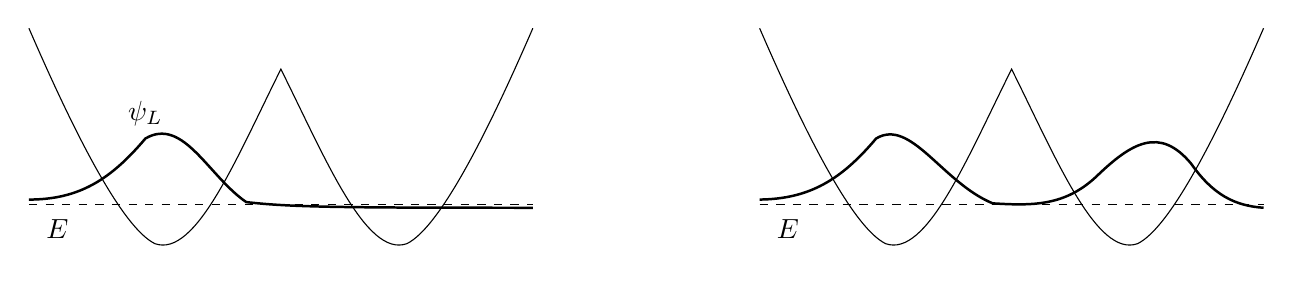
\begin{tikzpicture}[x=0.8cm,y=0.8cm]
\begin{scope}[shift={(-5.8,0)}]
\draw (-4,2.7) .. controls (-3.35,1.2) and (-2.55,-0.45) .. (-2.0,-0.72)
      .. controls (-1.35,-0.95) and (-0.7,0.65) .. (0,2.05)
      .. controls (0.7,0.65) and (1.35,-0.95) .. (2.0,-0.72)
      .. controls (2.55,-0.45) and (3.35,1.2) .. (4,2.7);
\draw[dashed] (-4,-0.10) -- (4,-0.10);
\node at (-3.55,-0.48) {$E$};
\draw[line width=0.9pt] (-4,-0.02) .. controls (-3.2,-0.02) and (-2.7,0.30) .. (-2.15,0.95)
      .. controls (-1.55,1.30) and (-1.15,0.35) .. (-0.55,-0.06)
      .. controls (0.15,-0.14) and (0.9,-0.15) .. (4,-0.15);
\node at (-2.15,1.35) {$\psi_L$};
\end{scope}
\begin{scope}[shift={(5.8,0)}]
\draw (-4,2.7) .. controls (-3.35,1.2) and (-2.55,-0.45) .. (-2.0,-0.72)
      .. controls (-1.35,-0.95) and (-0.7,0.65) .. (0,2.05)
      .. controls (0.7,0.65) and (1.35,-0.95) .. (2.0,-0.72)
      .. controls (2.55,-0.45) and (3.35,1.2) .. (4,2.7);
\draw[dashed] (-4,-0.10) -- (4,-0.10);
\node at (-3.55,-0.48) {$E$};
\draw[line width=0.9pt] (-4,-0.02) .. controls (-3.2,-0.01) and (-2.7,0.30) .. (-2.15,0.95)
      .. controls (-1.6,1.28) and (-1.1,0.25) .. (-0.30,-0.08)
      .. controls (0.35,-0.12) and (0.85,-0.12) .. (1.35,0.35)
      .. controls (1.9,0.88) and (2.35,1.15) .. (2.85,0.55)
      .. controls (3.2,0.05) and (3.55,-0.12) .. (4,-0.15);
\end{scope}
\end{tikzpicture}
\end{adjustbox}
\caption{칠판에 처음 그린 스케치를 깔끔하게 다시 그린 그림이다. 왼쪽은 장벽이 사실상 무한히 높다고 가정해 얻은 한쪽짜리 시험 상태 \(\psi_L\)이다. 오른쪽은 같은 파동함수를 장벽 너머로 대칭적으로 연장한 것으로, 실제 짝대칭 바닥 상태를 결국 만들어 내는 작지만 영이 아닌 누설을 보여 준다.}
\end{figure}

하지만 양자역학적으로 장벽은 실제로 무한대가 아닙니다. 장벽 영역의 파동함수는 정확히 0이 아니라 아주 작을 뿐입니다. 이 미세한 누설이 전부입니다. 이 누설 때문에 좌우 근사가 실제 혼합 문제로 바뀝니다.

\section{패리티 고유상태와 지수적 에너지 준위 분리}

이제 국소화된 상태에 관한 설명을 정리하는 정리가 나옵니다. 퍼텐셜이 대칭이면 정확한 에너지 고유함수는 반사에 대해 대칭이거나 반대칭이 되도록 선택할 수 있습니다.

\begin{theorem}
1차원에서 \(V(x)=V(-x)\)이면 해밀토니안의 고유함수는 다음 중 하나를 만족하도록 선택할 수 있습니다.
\[
\psi(x)=\psi(-x)
\qquad \text{or} \qquad
\psi(x)=-\psi(-x).
\]
\end{theorem}

이제 보정이 필요합니다. 한쪽에 국소화된 상태 \(\psi_L\)와 \(\psi_R\)는 대칭도 반대칭도 아니므로 전체 해밀토니안의 정확한 고유상태일 수 없습니다. 이 상태들은 장벽이 높을 때만 좋은 근사 상태입니다. 진정한 고유상태는 대칭 및 반대칭 결합입니다.
\begin{align}
\psi_+ &= \frac{\psi_L+\psi_R}{\sqrt{2}},\\
\psi_- &= \frac{\psi_L-\psi_R}{\sqrt{2}}.
\end{align}
칠판에서 계속 쓸 표기법으로 두 상태의 에너지를 다음과 같이 표시하겠습니다.
\begin{align}
H\psi_+ &= (E_1-\epsilon)\psi_+,\\
H\psi_- &= (E_1+\epsilon)\psi_-.
\end{align}
따라서 전체 준위 분리는
\begin{equation}
\Delta E = (E_1+\epsilon)-(E_1-\epsilon)=2\epsilon .
\end{equation}

\begin{figure}[htbp]
\centering
\includegraphics[width=0.92\linewidth]{lecture_08_frame_02.png}
\caption{이중 우물 퍼텐셜에서 대칭적으로 연장한 파동함수이다. 장벽 아래에서도 진폭은 작지만 영이 아니며, 이것이 에너지 준위 분리의 원인이다.}
\lectureframe{00:06:19}
\end{figure}

\begin{figure}
\centering
\begin{tikzpicture}[x=1cm,y=1cm]
\draw[->] (0,0) -- (0,3);
\node[left] at (0,2.8) {energy};
\draw (-0.35,1.60) -- (0.35,1.60);
\node[left] at (-0.45,1.60) {$\psi_L,\psi_R$};
\node at (1.7,1.60) {$\Longrightarrow$};
\draw (3.0,1.32) -- (3.75,1.32);
\draw (3.0,1.88) -- (3.75,1.88);
\draw[dashed] (2.8,1.60) -- (3.95,1.60);
\node[right] at (3.9,1.32) {$\psi_+,\ E_1-\epsilon$};
\node[right] at (3.9,1.88) {$\psi_-,\ E_1+\epsilon$};
\node[below] at (3.37,1.60) {$E_1$};
\end{tikzpicture}
\caption{터널링에 의한 에너지 분리의 칠판 설명. 근사적인 왼쪽 및 오른쪽 상태는 거의 축퇴되어 있지만, 정확한 대칭 및 반대칭 고유상태는 작은 양 \(2\epsilon\)만큼 에너지가 갈라져 있다.}
\end{figure}

준위의 순서에 물리적 요점이 담겨 있습니다. 대칭 상태는 장벽 영역에서 파동함수가 더 매끄럽게 이어지므로 에너지가 약간 더 낮습니다. 파동함수가 새어 나와 대칭적으로 이어지도록 허용하면 에너지가 아주 조금 내려갑니다. 반대칭 상태는 약간 더 높은데, 1차원 첫 번째 여기 상태에는 마디가 하나 있고 이 대칭 문제에서는 그 마디가 중심점에 놓이기 때문입니다. 곡률이 더 커지면 운동에너지가 증가합니다.

이 효과는 매우 작으며 장벽의 폭과 높이에 따라 지수적으로 작아집니다. 여기서는 명시적인 WKB 공식을 쓸 필요가 없습니다. 중요한 점은 준위 분리가 실제로 있지만 아주 작다는 것입니다. 또한 파동함수의 전체 부호에는 물리적 의미가 없다는 것을 기억하세요. \(\psi_-\)를 \(-\psi_-\)로 바꾸어도 상태는 달라지지 않습니다.

\section{시간 진화와 좌우 진동}

이제 동역학적 질문을 해 봅시다. 입자를 왼쪽 우물에 놓으면 어떻게 될까요? 진동은 같은 혼합 현상이 시간에 따라 나타나는 모습이므로, 이것이 결정적인 단계입니다.

역관계는 다음과 같습니다.
\begin{align}
\psi_L &= \frac{\psi_+ + \psi_-}{\sqrt{2}},\\
\psi_R &= \frac{\psi_+ - \psi_-}{\sqrt{2}}.
\end{align}
따라서 처음에 왼쪽에 국소화된 상태는
\begin{equation}
\psi(0)=\psi_L=\frac{\psi_+ + \psi_-}{\sqrt{2}}.
\end{equation}
에너지 고유상태가 아니므로 비자명하게 시간에 따라 진화해야 합니다.

표준 Schr\"odinger 규약 \(e^{-iEt}\)을 사용하겠습니다. 공통 위상은 관측 가능한 효과가 없습니다. 한 우물에서 다른 우물로 확률을 옮길 수 있는 것은 두 에너지 성분 사이의 상대 위상뿐입니다.

이 규약에 따르면,
\begin{equation}
\psi(t)=\frac{1}{\sqrt{2}}\left(e^{-i(E_1-\epsilon)t}\psi_+ + e^{-i(E_1+\epsilon)t}\psi_-\right).
\end{equation}
이것은 칠판 공식을 정리한 형태입니다. 이제 공통 위상을 묶어 내면,
\begin{equation}
\psi(t)=\frac{e^{-iE_1 t}}{\sqrt{2}}\left(e^{i\epsilon t}\psi_+ + e^{-i\epsilon t}\psi_-\right).
\end{equation}
이제 한 위상은 단위원 위에서 한 방향으로 진행하고 다른 위상은 반대 방향으로 진행합니다. 두 위상이 서로 어긋나기 때문에 상태가 변합니다.

좌우 진동을 명시적으로 확인하려면 \(\psi_\pm\)의 정의를 대입합니다.
\begin{align}
\psi(t)
&= \frac{e^{-iE_1 t}}{2}
\left[e^{i\epsilon t}(\psi_L+\psi_R)+e^{-i\epsilon t}(\psi_L-\psi_R)\right] \\
&= \frac{e^{-iE_1 t}}{2}
\left[(e^{i\epsilon t}+e^{-i\epsilon t})\psi_L+(e^{i\epsilon t}-e^{-i\epsilon t})\psi_R\right] \\
&= e^{-iE_1 t}\left[\psi_L\cos(\epsilon t)+i\,\psi_R\sin(\epsilon t)\right].
\end{align}
이것이 이 장의 핵심 유도 과정입니다. \(\psi_L\)와 \(\psi_R\)가 정규직교인 2상태 근사에서 확률은 다음과 같습니다.
\begin{equation}
P_L(t)=\cos^2(\epsilon t),
\qquad
P_R(t)=\sin^2(\epsilon t).
\end{equation}
따라서 계는 진동합니다. 중간 시간에는 실제로 중첩 상태에 있습니다. 예를 들어 \(\epsilon t=\pi/4\)일 때 양쪽의 확률은 같습니다. 위상은 연속적으로 진화하고, 국소화도 그에 따라 연속적으로 변합니다.

칠판 유도에서는 상대 부호가 처음 뒤집히는 시간을 찾습니다. 다음 조건을 만족하는 때를 구합니다.
\begin{equation}
e^{-i\epsilon t}=-\,e^{i\epsilon t},
\end{equation}
이것이 칠판에 표시된 눈에 띄는 시점입니다. 양변을 정리하면
\begin{equation}
e^{2i\epsilon t}=-1.
\end{equation}
첫 번째로 성립하는 때는
\begin{equation}
2\epsilon t=\pi,
\qquad\text{so}\qquad
t_{L\to R}=\frac{\pi}{2\epsilon}.
\end{equation}

\begin{figure}[htbp]
\centering
\includegraphics[width=0.94\linewidth]{lecture_08_frame_05.png}
\caption{칠판의 상대 위상 계산. \(e^{2i\epsilon t}=-1\)일 때 두 에너지 성분의 부호가 반대가 되어 첫 번째 전이 시간 \(2\epsilon t=\pi\)을 얻는다. 식으로 쓴 유도에서는 일관된 Schr\"odinger 위상 규약 하나를 사용한다.}
\lectureframe{00:17:52}
\end{figure}
그 순간에는,
\begin{equation}
\psi(t_{L\to R}) \propto \frac{\psi_+-\psi_-}{\sqrt{2}}=\psi_R.
\end{equation}
전체 위상은 중요하지 않습니다. 중요한 것은 처음에 왼쪽에 놓인 입자가 오른쪽에 국소화된 상태로 진화했다는 점입니다. 같은 시간이 한 번 더 지나면 다시 되돌아옵니다. 혼합과 진동은 함께 나타납니다.

방정식은 분명합니다. \(\epsilon\)가 작으면 진동이 느리고 전이 시간은 깁니다. 두 국소화 상태 어느 쪽도 에너지가 정해져 있지 않지만, 두 정확한 에너지 성분은 에너지를 보존하며 정확히 예상대로 진화합니다.

\section{중성미자, 암모니아와 스핀 유사성}

이중 우물은 처음의 중성미자 질문을 이해할 틀을 제공합니다. 전자와 함께 생성된 중성미자를 전자 중성미자라고 하고, 뮤온과 함께 생성된 중성미자를 뮤온 중성미자라고 합니다. 이 향미 표지는 생성 및 검출 채널을 나타냅니다. 질량이 정해진 상태, 따라서 운동량이 고정된 자유 입자 에너지가 정해진 상태들은 또 다른 기저를 이룹니다.

가장 단순한 두 상태 최대 혼합 모형에서는,
\begin{equation}
|\nu_e\rangle \sim \frac{|m_1\rangle+|m_2\rangle}{\sqrt{2}},
\qquad
|\nu_\mu\rangle \sim \frac{|m_1\rangle-|m_2\rangle}{\sqrt{2}},
\end{equation}
여기서 질량 고유상태는 \(\psi_+\) 및 \(\psi_-\)의 역할을 하고, 향미 상태는 \(\psi_L\) 및 \(\psi_R\)의 역할을 합니다. 실제 중성미자 혼합에는 이와 같은 동일 계수 대신 비자명한 혼합 행렬이 쓰이지만, 여기서도 메커니즘은 이미 드러납니다.

전자 중성미자는 전자가 관여하는 과정에서 생성되며, 이는 입자를 왼쪽 우물에 넣는 것과 비슷합니다. 짧은 거리를 이동하는 동안 두 질량 성분은 거의 같은 위상을 얻으므로, 상호작용에서 여전히 전자 향미로 식별됩니다. 긴 거리를 지나면 두 성분의 위상이 갈라집니다. 이후의 하전 전류 상호작용에서는 전자 대신 뮤온이 생성될 수 있습니다. 즉, 상태에 뮤온 향미 성분이 생긴 것입니다. 거리가 다르거나 에너지가 다른 조건에서 실험을 반복하면 진동을 확인할 수 있습니다.

에너지 보존과 충돌하지 않습니다. 질량-에너지 고유상태는 고유상태에 기대되는 대로 정확히 거동합니다. 진화하는 것은 향미 중첩입니다. 상대론적 극한에서 관측 가능한 상대 위상은 개략적으로 질량 제곱 차이로 결정됩니다.
\begin{equation}
\Delta\phi_{ij}\simeq \frac{\Delta m_{ij}^{,2}L}{2E}.
\end{equation}
따라서 진동은 중성미자 질량이 모두 같을 수 없음을 보여 줍니다. 적어도 두 질량 고유상태의 질량은 서로 다릅니다.

\begin{classroomqa}
\lecturetimestamp{00:24:06}
\audiencequestion{이중 우물 사례에서 작은 준위 분리 \(\epsilon\)는 무엇으로 결정되나요?}
\lecturerresponse{입자의 질량과 장벽의 높이 및 폭에 따라 달라집니다. 터널링은 이런 세부 조건에 지수적으로 민감하므로, 장벽이 조금만 달라져도 \(\epsilon\)는 비율상 크게 달라질 수 있습니다.}
\end{classroomqa}

\begin{classroomqa}
\lecturetimestamp{00:24:26}
\audiencequestion{이런 진동 현상은 실제로 관측되었나요?}
\lecturerresponse{그렇습니다. 보통의 양자계에서 터널링에 의한 준위 분리가 관측되고, 중성미자의 향미 진동도 관측됩니다. 미시적인 메커니즘은 다르지만 둘 다 같은 2상태 위상 진화를 구현합니다.}
\end{classroomqa}

\begin{classroomqa}
\lecturetimestamp{00:24:34}
\audiencequestion{중성미자 진동은 중성미자 질량과 어떻게 연결되나요?}
\lecturerresponse{전파하는 고유상태들의 질량이 서로 다르므로 서로 다른 위상을 얻습니다. 이들의 간섭으로 향미 구성이 변합니다. 현실적인 상대론적 설명에서 진동을 결정하는 것은 한 입자의 질량이 시간에 따라 실제로 변하는 것이 아니라 질량 제곱 차이입니다.}
\end{classroomqa}

\begin{classroomqa}
\lecturetimestamp{00:25:02}
\audiencequestion{중성미자 질량은 단지 통설일 뿐인가, 아니면 실험으로 확인된 사실인가?}
\lecturerresponse{중성미자 진동은 실험적 사실이며, 질량 차이가 영이 아니어야 진동이 일어난다. 절대 질량 척도는 별개의 문제이고 측정하기도 더 어렵지만, 모든 중성미자가 질량이 없다는 최소 모형은 실험적으로 배제되었다.}
\end{classroomqa}

\subsection{암모니아 반전: 실제 장벽}

암모니아 분자 \(\mathrm{NH}_3\)는 삼각뿔 구조입니다. 수소 원자 세 개가 한 평면을 이루고 질소 원자는 그 평면의 한쪽에 있습니다. 질소 원자가 반대쪽에 있는 등가 구조도 있습니다. 이 두 국소화 구조는 정확한 정상 상태가 아닙니다. 질소 원자는 수소 평면을 통과해 터널링할 수 있으며, 이로써 대칭 및 반대칭 에너지 고유상태와 작은 반전 에너지 분리가 생깁니다. 암모니아 메이저에서도 같은 수학적 구조가 나타나는 물리적 원인이 바로 이것입니다.

\begin{classroomqa}
\lecturetimestamp{00:25:11}
\audiencequestion{암모니아에서 장벽은 질소 원자가 수소 평면을 통과하는 구조인가요?}
\lecturerresponse{그렇습니다. 분자 에너지는 두 삼각뿔 구조 각각에서 최소가 되고 평면 구조에서는 더 높습니다. 이 구조를 통과하는 터널링이 양쪽을 결합합니다.}
\end{classroomqa}

\begin{classroomqa}
\lecturetimestamp{00:27:10}
\audiencequestion{전자 중성미자와 뮤온 중성미자 사이에 대응하는 물리적 장벽은 무엇인가요?}
\lecturerresponse{실제 공간상의 장벽은 없습니다. 유사성은 대수적인 것입니다. 중성미자 해밀토니안의 비대각 결합이 향미 기저를 혼합합니다. 암모니아에서는 이 결합이 터널링에서 생기지만, 중성미자에서는 질량과 혼합 구조의 일부입니다.}
\end{classroomqa}

\subsection{스핀 세차: 터널링 없는 혼합}

스핀에서도 같은 대수적 구조를 이미 보았습니다. 두 상태 \(|\uparrow_z\rangle\)와 \(|\downarrow_z\rangle\)를 생각해 봅시다. 자기장이 없으면 두 상태는 축퇴되어 있습니다. 이제 \(x\) 방향으로 자기장을 켭니다. 에너지 고유상태는 더 이상 \(z\) 고유상태가 아니라 \(x\) 방향으로 편극된 상태입니다. 칠판에서 임시로 쓴 왼쪽--오른쪽 표기를 사용하면,
\begin{align}
|L_x\rangle &= \frac{|\uparrow_z\rangle+|\downarrow_z\rangle}{\sqrt{2}},\\
|R_x\rangle &= \frac{|\uparrow_z\rangle-|\downarrow_z\rangle}{\sqrt{2}}.
\end{align}
이들은 \(\psi_+\)와 \(\psi_-\)에 직접 대응합니다. 자기장과 나란하거나 반대인 자기 모멘트는 에너지가 조금 다릅니다. 두 에너지가 \(E\mp\epsilon\)라면 처음에 위쪽을 향한 스핀은 다음과 같이 진화합니다.
\begin{equation}
|\uparrow_z,t\rangle
= e^{-iEt}\left[\cos(\epsilon t)\,|\uparrow_z\rangle
+ i\sin(\epsilon t)\,|\downarrow_z\rangle\right].
\end{equation}
이 식은 이중 우물의 식과 같으며, 여기서는 \(x\)축을 중심으로 하는 스핀 세차가 연속적인 진화에 해당합니다. \(+z\)에서 시작한 스핀은 횡방향을 지나 반 바퀴 세차한 뒤 \(-z\)에 도달하고, 다시 반 바퀴 세차하면 돌아옵니다. \(S_z\)를 측정하면 여전히 위 또는 아래만 나오지만, 연속적으로 변하는 스핀 상태가 각 결과의 확률을 결정합니다. 이 메커니즘에는 터널링이 필요하지 않습니다. 준비 기저와 다른 기저에서 해밀토니안이 대각이기만 하면 됩니다.

\begin{classroomqa}
\lecturetimestamp{00:32:25}
\audiencequestion{이 그림에서 타우 중성미자는 어떻게 되나요?}
\lecturerresponse{타우 중성미자도 혼합됩니다. 실제 문제에는 향미 상태가 세 개이고 질량 상태도 세 개이므로, 2상태 회전 대신 3×3 혼합 행렬을 사용합니다. 위상 간섭 원리는 그대로입니다.}
\end{classroomqa}

\begin{classroomqa}
\lecturetimestamp{00:32:57}
\audiencequestion{횡방향 자기장을 걸고 바로 뒤에도 스핀은 여전히 위쪽을 향하나요? 우리 쪽이나 반대쪽을 향할 수도 있나요?}
\lecturerresponse{아주 짧은 시간이 지난 뒤에는 여전히 거의 확실히 위쪽을 향하며, 아래쪽일 확률은 작습니다. 스핀 상태는 자기장 축 주위로 연속적으로 세차하며 횡방향 \(\pm y\)을 지나갑니다. 처음에 자기장과 수직이었다면 \(x\) 방향 자기장에 대해서 계속 수직을 유지합니다. 어느 축을 선택해 측정하더라도 그 축의 이산적인 고유값 중 하나가 나옵니다.}
\end{classroomqa}

\begin{classroomqa}
\lecturetimestamp{00:34:30}
\audiencequestion{스핀이 자기장 방향을 향하지 않도록 약한 자기장을 선택한 건가요?}
\lecturerresponse{아닙니다. 스핀의 기하학적 거동은 자기장의 세기가 아니라 자기장 축 주위의 세차로 결정됩니다. 약한 자기장은 에너지 분리와 세차 주파수를 작게 만들어 진동을 느리게 할 뿐이며, 이는 중성미자 사례와 비슷합니다.}
\end{classroomqa}

중성미자 혼합의 세기와 작은 중성미자 질량은 원래의 최소 표준 모형으로는 그 더 깊은 기원을 설명할 수 없는 매개변수입니다. 따라서 중성미자 질량은 그 최소 모형 너머의 물리를 가리킵니다. 다만 관측된 질량 척도는 매우 작으며, 먼 에너지 척도의 물리를 반영할 수도 있습니다.

\begin{classroomqa}
\lecturetimestamp{00:36:27}
\audiencequestion{중성미자에 질량이 있다는 것을 알게 된 근거가 진동인가요?}
\lecturerresponse{전파하는 성분들의 질량이 서로 다르다는 결정적인 직접 증거입니다. 관련 성분들이 모두 정확히 질량이 없고 축퇴되어 있다면 질량에 따른 상대 위상을 얻지 않을 것이며, 이런 종류의 진공 향미 진동은 일어나지 않을 것입니다.}
\end{classroomqa}

\begin{classroomqa}
\lecturetimestamp{00:37:57}
\audiencequestion{반주기에는 중성미자가 전자 맛과 뮤온 맛을 절반씩 띠어야 하는가?}
\lecturerresponse{이상적인 대칭 두 상태 모형에서는 전체 확률 주기의 사분의 일 지점에서 두 맛을 관측할 확률이 같고, 첫 번째 최댓값에서 완전히 전환된다. 실제 세 가지 맛의 진동에서는 혼합각이 서로 다르고 진동수가 여러 개이며, 스핀·헬리시티 제약과 물질 효과도 있으므로 대칭적인 완전 전환은 일반적이지 않다.}
\end{classroomqa}

\begin{classroomqa}
\lecturetimestamp{00:38:36}
\audiencequestion{질량 성분이 다르다면 태양 중성미자가 운동량을 보존하려면 속도가 변해야 하나요?}
\lecturerresponse{향미 상태는 질량이 고정된 성분들의 결맞은 중첩입니다. 그 상태의 질량이 고전적 양처럼 시간에 따라 진동하는 것은 아닙니다. 운동량이 같은 것으로 기술하는 일반적인 방식에서는 성분들의 에너지와 군속도가 조금씩 다릅니다. 에너지가 같은 방식에서는 운동량이 조금씩 다릅니다. 두 규약 모두 일관되게 적용하면 같은 관측 가능한 진동 위상을 줍니다.}
\end{classroomqa}

이 위상 진화로 과거의 태양 중성미자 부족 문제가 해소되었습니다. 초기 검출기는 주로 전자 중성미자에 민감했으므로, 태양을 전자 향미로 떠난 중성미자는 뮤온 또는 타우 향미로 일부 도달해 해당 검출 채널에서 빠져나갈 수 있었습니다. 태양 중성미자를 자세히 계산할 때는 3향미 혼합과 물질 효과를 포함하지만, 개념적 교훈은 이미 이중 우물에 담겨 있습니다. 준비와 전파에는 서로 다른 기저가 쓰입니다.

\section{삽화: 전기 쌍극자 모멘트, 대칭성과 ``전자 구체'' 주장}

입자 현상론을 이야기하고 있으니 형식적 수학에서 잠시 벗어나 봅시다. 한 대중 매체 기사는 전자의 전기 쌍극자 모멘트 상한이 새로 측정되었다는 내용을 전자가 구형임이 밝혀졌다는 말로 소개했습니다. 이 표어는 서로 다른 세 가지 질문을 혼동합니다. 전기 쌍극자 모멘트가 무엇을 측정하는지, 양자 상태에서 회전 대칭성이 무엇을 뜻하는지, 그리고 실험이 실제로 무엇을 제한했는지입니다.

\subsection{무엇을 측정했나?}

측정된 것, 더 정확히는 상한만 정해진 것은 전자의 전기 쌍극자 모멘트이다. 전하 \(\pm q\)가 서로 떨어져 있을 때 쌍극자 모멘트는
\begin{equation}
\mathbf d = q\,\boldsymbol{\ell},
\end{equation}
이며, \(\boldsymbol{\ell}\)는 분리 벡터이다. 영이 아닌 쌍극자 모멘트는 전하 분포가 어떤 중심에 대해 치우쳐 있음을 뜻한다.

하지만 전자의 경우 중요한 질문은 전하가 임의의 어떤 방향으로 중심에서 벗어나 있는지에 그치지 않습니다. 전자에는 스핀이 있으므로 축이 있습니다. 자기 모멘트도 있습니다. 물리적으로 의미 있는 질문은 전하의 변위와 그 축 사이에 상관관계가 있는가입니다.
\begin{equation}
\mathbf d_e \parallel \boldsymbol{\mu}_e
\qquad \text{or equivalently} \qquad
\mathbf d_e \parallel \mathbf S .
\end{equation}
이 상관관계를 전자의 전기 쌍극자 모멘트라고 합니다. 개념적으로는 스핀 편극된 전자를 전기장에 놓았을 때 두 스핀 방향의 에너지가 갈라지는지를 묻습니다.
\begin{equation}
H_{\mathrm{EDM}}=-\mathbf d_e\cdot \mathbf E,
\qquad
\mathbf d_e=d_e\frac{\mathbf S}{|\mathbf S|}.
\end{equation}
실제 탁상 실험은 전자를 축전기 판 사이에 그냥 놓는 것보다 훨씬 정교하지만, 이 실험이 이용하는 대칭성과 에너지 이동의 핵심은 바로 이것입니다.

\subsection{전기 쌍극자 모멘트가 없어도 구형이라는 뜻은 아니다}

첫 번째로 바로잡을 점은 간단합니다. 물체에 쌍극자 모멘트가 없어도 구형이 아닐 수 있습니다. 중심이 맞춰진 타원체는 한쪽과 다른 쪽의 전하량이 같아 쌍극자 모멘트가 없지만, 사중극자 모멘트는 가질 수 있습니다. 더 복잡한 분포는 쌍극자 모멘트와 사중극자 모멘트가 모두 없어도 더 높은 다중극 모멘트를 가질 수 있습니다. 다중극 계수 하나를 측정한다고 전체 모양이 정해지는 것은 아닙니다.

양자역학에서는 ``모양''이라는 말이 더 미묘해집니다. 결합 길이가 거의 고정된 두 원자 분자, 즉 아령처럼 생긴 분자를 생각해 봅시다. 반지름 방향 진동은 무시하고 회전만 고려합니다. 이 분자의 회전 상태는 각운동량으로 표시합니다. 분자가 보손이면 가장 낮은 회전 상태는 \(J=0\)입니다. 각운동량이 회전을 생성하므로,
\begin{equation}
\begin{gathered}
J=0 \quad\Longrightarrow\\
\text{rotationally invariant ground state.}
\end{gathered}
\end{equation}
모든 특정 방향의 그림은 아령처럼 보이지만 양자 상태는 회전에 대해 불변입니다. 이 상태를 모든 방향이 결맞게 중첩된 상태로 설명할 수도 있습니다. 상태를 ``구형''이라고 부르는 것은 어떤 측정에는 유용하지만 다른 측정에는 오해를 낳습니다.

짧은 순간을 포착해 봅시다. 순간 포착은 방향을 측정하는 것으로, 방향을 충분히 정밀하게 측정하면 계는 각도상 국소화된 상태로 남습니다. 이런 상태는 각운동량도 동시에 정해져 있을 수 없습니다. 이는 위치--운동량 불확정성 원리의 회전 버전입니다. 각도를 국소화하면 각운동량이 필연적으로 퍼지고, 따라서 회전 여기 상태가 생깁니다.

강체 회전자의 경우,
\begin{equation}
E_J=\frac{J(J+1)}{2I},
\end{equation}
따라서 분해능을 정하는 에너지는 관성 모멘트 \(I\)에 좌우됩니다. 체육관에서 쓰는 아령은 \(I\)가 매우 커 회전 준위 간격이 터무니없이 좁습니다. 보통의 빛만으로도 방향이 드러날 만큼 쉽게 교란할 수 있습니다. 분자에서는 준위 간격이 더 넓습니다. 크기가 작은 강입자에서는 그 간격이 훨씬 더 넓습니다. 탐침 에너지가 처음으로 분해할 수 있는 회전 구조를 들뜨게 하기에 부족하다면, 반복 측정에서도 회전 평균을 낸 바닥상태만 관측됩니다.

중간자는 대략 쿼크--반쿼크의 2체 계로 그려 볼 수 있습니다. 첫 번째 궤도 여기에는 수억 전자볼트 이상의 에너지가 필요하며, 광학 광자의 에너지보다 훨씬 큽니다. 따라서 저에너지 탐침으로는 내부 방향을 순간 포착할 수 없습니다. ``구형인가 아닌가''라는 질문은 어떤 상태를 준비하느냐의 문제이기도 하고 장치의 분해능에 관한 문제이기도 합니다.

전자를 보면 문제가 더 분명해진다. 전자는 스핀-\(\tfrac12\) 입자이지 회전 스칼라가 아니다. 스핀이 편극된 상태는 축과 자기 모멘트를 갖는다. 그 축을 따라 전하가 회전한다는 익숙한 그림은 어디까지나 직관적 설명이다---점입자인 디랙 입자가 실제로 작은 회전 구라는 뜻은 아니다---하지만 자기 모멘트가 스핀과 함께 방향을 바꾼다는 점을 올바르게 일깨워 준다. 전기 쌍극자 모멘트에 관한 질문은 전하의 변위가 바로 그 축과 상관되어 있는지를 묻는다. 답이 영이라고 해서 전자가 고전적인 구가 되는 것은 아니다.

\begin{classroomqa}
\lecturetimestamp{00:57:30}
\audiencequestion{전자 전하의 일부를 옮기면 전하 양자화에 어긋나나요?}
\lecturerresponse{아닙니다. 전하 양자화가 정하는 것은 전체 전하입니다. 쌍극자 모멘트는 전하 분포의 공간에 대한 1차 모멘트이거나, 동등하게 말해 전기장에 대한 허용된 점입자 결합입니다. 전체 전하가 분수만큼 바뀌어야 하는 것은 아닙니다.}
\end{classroomqa}

\begin{classroomqa}
\lecturetimestamp{00:58:00}
\audiencequestion{양자장론에서는 전기 쌍극자 모멘트가 금지되나요?}
\lecturerresponse{양자장론 자체가 금지하는 것은 아닙니다. 특정 이산 대칭이 정확하게 성립할 때 금지됩니다. 그런 대칭이 깨지면 전기 쌍극자 모멘트 연산자가 허용되지만, 그 계수는 극도로 작을 수 있습니다.}
\end{classroomqa}

\subsection{패리티와 시간 반전}

전기 쌍극자 모멘트 논의의 핵심은 대칭성이다. 패리티 변환에서 전기 쌍극자 모멘트는 보통 극벡터처럼 변환되는 반면, 자기 모멘트는 축벡터처럼 변환된다:
\begin{align}
P:\qquad &\mathbf d_e \to -\mathbf d_e,
&\boldsymbol{\mu}_e \to \boldsymbol{\mu}_e .
\end{align}
시간 반전에서는 자기 모멘트를 정의하는 순환 전류가 반전되지만, 정적인 전기 변위는 그렇지 않다:
\begin{align}
T:\qquad &\mathbf d_e \to \mathbf d_e,
&\boldsymbol{\mu}_e \to -\boldsymbol{\mu}_e .
\end{align}
따라서 전자의 스핀 축에 정렬된 영이 아닌 전기 쌍극자 모멘트는 패리티 대칭이 정확히 성립할 때 금지되며, 시간 반전 대칭이 정확히 성립할 때도 금지된다:
\begin{equation}
(P\ \text{exact}) \Rightarrow \mathbf d_e=0,
\qquad
(T\ \text{exact}) \Rightarrow \mathbf d_e=0.
\end{equation}

기하학적 내용을 명확히 짚어 보자. 자기 모멘트는 고리 모양의 전류가 만들어 낸다. 거울 반사는 보통의 극벡터 방향을 뒤집지만, 그 고리에 수직인 축벡터는 그대로 둔다. 반면 전하 변위는 축을 따라 반전된다. 따라서 \(\mathbf d_e\)가 \(\boldsymbol\mu_e\)와 평행한 전자는 거울 반사하면 자기 방향은 같지만 전기 모멘트와 자기 모멘트의 상대적 방향은 반대인 전자로 바뀐다. 패리티가 정확한 대칭이고 전자 종류가 하나뿐이라면 두 기술은 같은 입자를 나타내야 한다. 이때 양립하는 것은 \(d_e=0\)뿐이다.

시간 반전도 다른 방식으로 같은 결론을 준다. 필름을 거꾸로 재생하면 전류가 반전되므로 \(\boldsymbol\mu_e\)도 반전되지만, 정지한 전하 변위는 움직이지 않는다. 평행한 모멘트를 가진 상태는 반평행 모멘트를 가진 상태로 바뀐다. 시간 반전 대칭이 정확하다면 여기서도 \(d_e=0\)여야 한다.

\begin{figure}[htbp]
\centering
\begin{tikzpicture}[>=Stealth,scale=0.95]
  \node[font=\bfseries] at (1.0,2.25) {original};
  \draw[->,very thick,blue!70!black] (0.65,0) -- (0.65,1.65);
  \draw[->,very thick,red!75!black] (1.35,0) -- (1.35,1.65);
  \node[blue!70!black,below] at (0.65,0) {$\boldsymbol\mu$};
  \node[red!75!black,below] at (1.35,0) {$\mathbf d$};

  \node[font=\bfseries] at (4.5,2.25) {parity};
  \draw[->,very thick,blue!70!black] (4.15,0) -- (4.15,1.65);
  \draw[->,very thick,red!75!black] (4.85,1.65) -- (4.85,0);
  \node[blue!70!black,below] at (4.15,0) {$\boldsymbol\mu$};
  \node[red!75!black,below] at (4.85,0) {$-\mathbf d$};

  \node[font=\bfseries] at (8.0,2.25) {time reversal};
  \draw[->,very thick,blue!70!black] (7.65,1.65) -- (7.65,0);
  \draw[->,very thick,red!75!black] (8.35,0) -- (8.35,1.65);
  \node[blue!70!black,below] at (7.65,0) {$-\boldsymbol\mu$};
  \node[red!75!black,below] at (8.35,0) {$\mathbf d$};
\end{tikzpicture}
\caption{칠판의 논증을 바탕으로 정리한 대칭성 검증. 패리티는 전기 쌍극자를 반전시키지만 축벡터인 자기 모멘트는 그대로 둔다. 시간 반전은 자기 모멘트를 반전시키지만 정지한 전기 변위는 그대로 둔다. 어느 대칭이든 정확하다면 스핀과 평행한 영구 EDM은 허용되지 않는다.}
\end{figure}

\begin{figure}[htbp]
\centering
\includegraphics[width=0.94\linewidth]{lecture_08_frame_06.png}
\caption{시간 반전 논증에 등장하는 자기축과 전하 변위의 짝을 이룬 스케치. 위의 간결한 TikZ 그림은 일부 지워진 실제 칠판에서 변환의 핵심 내용만 분리해 보여 준다.}
\lectureframe{01:06:10}
\end{figure}

\begin{classroomqa}
\lecturetimestamp{01:06:38}
\audiencequestion{시간 반전에서 전류와 전하가 모두 반전되나요?}
\lecturerresponse{속도가 반전되므로 전류는 반전되지만, 전하 자체는 반전되지 않습니다. 전하의 부호를 반전시키는 것은 시간 반전 \(T\)이 아니라 전하 켤레 변환 \(C\)입니다.}
\end{classroomqa}

\begin{classroomqa}
\lecturetimestamp{01:07:01}
\audiencequestion{시간 반전이 반유니터리라는 것은 비상대론적 양자역학이 시간 반전 대칭을 갖지 않는다는 뜻인가요?}
\lecturerresponse{아닙니다. 반유니터리성은 양자역학에서 시간 반전을 일관되게 나타내는 바로 그 방식입니다. 시간 반전은 진폭을 복소켤레화하고 운동량과 스핀을 반전시킵니다. 특정 해밀토니안이 대칭을 갖는지는 별개의 문제입니다.}
\end{classroomqa}

\begin{classroomqa}
\lecturetimestamp{01:07:19}
\audiencequestion{EDM을 논하려면 전자가 점입자가 아니라 유한한 부피를 가져야 하나요?}
\lecturerresponse{아닙니다. 점입자 유효 해밀토니안에도 \(-d_e\,\widehat{\mathbf S}\!\cdot\!\mathbf E\)가 들어갈 수 있습니다. 실험에서는 스핀 방향이 반대일 때 전기장 속 에너지가 달라지는지를 묻습니다. 실제로 확장된 전하 분포가 있는지를 분해해 관측할 필요는 없습니다.}
\end{classroomqa}

패리티는 약한 상호작용의 대칭성이 아니며, 약한 상호작용의 카이랄 결합에서는 가능한 한 크게 위반된다. 시간 반전 대칭도 정확히 성립하지는 않지만, 표준 모형에서 알려진 시간 반전 위반이 전자 전기쌍극자 모멘트에 미치는 영향은 극도로 작다. 표준 모형의 기여가 영이 아님을 계산으로 보일 수는 있지만, 그 크기는 여기서 논의하는 민감도보다 훨씬 낮다. 따라서 검출되지 않은 결과는 표준 모형과 양립하면서, 확장 이론---, 예컨대 초대칭과 훨씬 큰 시간 반전 위반을 일으킬 수 있는 다른 새로운 상호작용---에 대한 제약을 강화한다.

기본적인 실험 발상은 간단하다. 자기장은 스핀 방향에 따른 에너지 분할을 통해 자기 쌍극자를 드러낸다. 전기장은 스핀과 상관된 추가 에너지 이동을 통해 EDM을 드러낼 수 있다. 실제 정밀 실험에서는 단순한 장치 속 고립 전자 대신 원자나 분자를 사용하고, 긴 결맞음 세차 시간을 확보하며, 인가한 장을 반전시키고 계통오차를 세심하게 제어한다.

\begin{classroomqa}
\lecturetimestamp{01:11:02}
\audiencequestion{EDM 탐색은 고에너지 충돌 실험이었나요, 아니면 물질을 이용한 실험이었나요?}
\lecturerresponse{전기장과 자기장을 함께 사용하고, 제어된 원자나 분자 환경에 속박된 전자를 이용한 탁상형 정밀 물리 실험이었습니다. 에너지는 낮지만, 대칭성 위반으로 생기는 미세한 에너지 이동을 민감하게 측정해 고에너지의 새로운 물리를 간접적으로 탐색합니다.}
\end{classroomqa}

\begin{classroomqa}
\lecturetimestamp{01:12:21}
\audiencequestion{검출되지 않았다는 결과는 표준 모형의 어떤 수정안이 여전히 가능할지 제약하는가?}
\lecturerresponse{원칙적으로는 그렇다. 모든 모형은 계수를 예측하므로 그에 따라 어떤 매개변수 영역을 차지한다. 구체적인 수치 배제 범위를 정하려면 전문적인 계산이 필요하지만, 일반적인 논리는 확고하다---정밀도가 높아질수록 표준 모형과의 일치가 커지므로, 큰 전기쌍극자 모멘트를 예측하는 대안이 들어설 여지는 줄어든다.}
\end{classroomqa}

\begin{classroomqa}
\lecturetimestamp{01:13:09}
\audiencequestion{양자 정보가 보존되려면 시간 반전 대칭이 필요한가요?}
\lecturerresponse{아닙니다. 해밀토니안이 \(T\)에 대해 불변이 아니더라도 유니터리 시간 발전은 정보를 보존합니다. 고정된 자기장 속 입자가 익숙한 예입니다. 시간을 거꾸로 재생한 영상에서 자기장도 함께 반전하지 않으면 자기장이 특정 시간 방향을 정하지만, 양자 시간 발전은 여전히 유니터리합니다. 국소적 로런츠 불변 양자장론의 통상적인 가정 아래에서는 결합 변환 \(CPT\)이 대칭이지만, 그것이 유니터리성을 보장하는 것은 아닙니다.}
\end{classroomqa}

이제 휴식은 끝내도 되겠다. 검출되지 않았다는 측정 결과는 명시된 민감도에서 전자의 전기쌍극자 모멘트가 검출되지 않았다는 뜻이다. 전자가 구형이라는 뜻도 아니고 표준 모형을 뒤엎는 것도 아니다. 다만 표준 모형에서 벗어난다는 몇몇 제안은 성립하기가 더 어려워진다.

\section{제2양자화로 돌아가기: 푸리에 변환, 운동량 모드, 국소성}

우리는 제2양자화를 다루고 있었다. 익숙한 단일 입자 파동함수의 성질부터 차근차근 다시 살펴본 다음, 이를 연산자로 확장하자. 푸리에 변환과의 연결은 정확하고 간단하다.

\subsection{위치 공간에서 운동량 공간으로}

대문자 \(\Psi\)가 아니라 소문자 \(\psi\)가 단일 입자의 파동함수다. 위치 공간에서
\begin{equation}
P(x)=|\psi(x)|^2
\end{equation}
는 위치 \(x\)에서 입자를 발견할 확률 밀도다. 운동량 공간의 파동함수는 그 푸리에 변환으로,
\begin{equation}
\tilde{\psi}(p)=\int dx\,\psi(x)\,\frac{e^{-ipx}}{\sqrt{2\pi}},
\end{equation}
역변환 관계는
\begin{equation}
\psi(x)=\int dp\,\tilde{\psi}(p)\,\frac{e^{ipx}}{\sqrt{2\pi}}.
\end{equation}
이다. 따라서
\begin{equation}
P(p)=|\tilde{\psi}(p)|^2
\end{equation}
는 운동량 \(p\)에 대한 확률 밀도다.

여기서는 \(\hbar=1\)를 사용한다. 두 변환은 서로 역변환이므로 어느 한 파동함수를 알면 다른 하나도 정해진다. 한편 각 파동함수의 절댓값 제곱은 서로 다른 측정 질문에 답한다.

자유 입자의 경우
\begin{equation}
H=\frac{p^2}{2m},
\end{equation}
이므로 운동량 고유상태는 에너지 고유상태이기도 하며, 이들의 위치 공간 파동함수는 평면파다.
\begin{equation}
\psi_p(x)\propto e^{ipx}.
\end{equation}
이것이 제2양자화에서 대응되는 논의를 시작하는 출발점이다.

\begin{figure}[htbp]
\centering
\includegraphics[width=0.94\linewidth]{lecture_08_frame_07.png}
\caption{한 입자 파동함수의 위치--운동량 푸리에 쌍. 소문자 \(\psi\)와 다음에 도입되는 대문자 장 연산자의 구별은 필수적이다.}
\lectureframe{01:20:00}
\end{figure}

\subsection{위치 공간과 운동량 공간의 장 연산자}

이제 장 연산자로 돌아가자. 칠판에서는 소멸 부분과 생성 부분을 \(\Psi_-(x)\) 및 \(\Psi_+(x)\)로 쓴다. 잠시 이 표기를 그대로 두면,
\begin{align}
\Psi_-(x) &= \sum_i a_i\,\psi_i(x),\\
\Psi_+(x) &= \sum_i a_i^\dagger\,\psi_i^*(x).
\end{align}
여기서 \(\psi_i(x)\)는 \(i\)번째 모드의 보통 단일 입자 파동함수이고, \(a_i\)와 \(a_i^\dagger\)는 그 모드의 입자를 각각 소멸시키고 생성한다. 이제부터는 다음과 같이 표기를 바꾸면 편리하다.
\[
\Psi(x)\equiv \Psi_-(x),
\qquad
\Psi^\dagger(x)\equiv \Psi_+(x).
\]

자유 입자에서는 이산 모드 지표 \(i\)를 연속적인 운동량 지표 \(p\)로 바꾼다. 평면파 \(e^{ipx}\)를 사용하면 표준적인 재구성 공식은 다음과 같다.
\begin{align}
\Psi(x) &= \int \frac{dp}{\sqrt{2\pi}}\,a(p)\,e^{ipx},\\
\Psi^\dagger(x) &= \int \frac{dp}{\sqrt{2\pi}}\,a^\dagger(p)\,e^{-ipx}.
\end{align}
이는 보통의 푸리에 변환에 대응하는 장 연산자 표현이다. 앞과 같은 방식으로 정확히 역변환할 수 있다.
\begin{align}
a(p) &= \int \frac{dx}{\sqrt{2\pi}}\,\Psi(x)\,e^{-ipx},\\
a^\dagger(p) &= \int \frac{dx}{\sqrt{2\pi}}\,\Psi^\dagger(x)\,e^{ipx}.
\end{align}
\(1/\sqrt{2\pi}\)의 계수는 정방향 변환과 역변환의 정규화가 같아지도록 택한 관례다.

개념적 내용은 간단하다. \(\Psi^\dagger(x)\)는 위치 \(x\)에서 입자를 생성하고, \(a^\dagger(p)\)는 운동량 \(p\)을 가진 입자를 생성한다. 위치 공간과 운동량 공간의 생성 연산자는 푸리에 켤레 관계이며, 보통의 양자역학에서 \(\psi(x)\)와 \(\tilde{\psi}(p)\)가 푸리에 켤레 관계인 것과 같다.

운동량 \(p\)를 가진 입자가 없다면 \(a(p)\)는 상태를 소멸시킨다. 그 운동량을 가진 입자가 있다면 통상적인 점유수 계수에 따라 입자 하나를 제거한다. 마찬가지로 \(\Psi(x)\)는 위치 \(x\)에서 입자를 제거하며, 이 연산은 분포의 의미로 이해하거나 파동묶음에 대해 스미어링한 뒤 이해한다. 입자 종류마다 고유한 장 연산자가 필요하다. 하나의 장이 모든 종류의 입자를 생성할 수는 없다.

\subsection{보손 교환자와 떨어진 곳에서의 측정 독립성}

다음 성질은 정의에서 직접 유도할 수 있다. 보손의 경우
\begin{equation}
[a_i,a_j^\dagger]=\delta_{ij},
\qquad
[a_i,a_j]=0,
\qquad
[a_i^\dagger,a_j^\dagger]=0.
\end{equation}
연속적인 경우에는
\begin{equation}
[a(p),a^\dagger(p')]=\delta(p-p').
\end{equation}
이다. 이제 이산 전개를 이용해 같은 시간의 장 교환자를 계산하면
\begin{align}
[\Psi(x),\Psi^\dagger(y)]
&= \sum_{i,j}\psi_i(x)\psi_j^*(y)\,[a_i,a_j^\dagger] \\
&= \sum_i \psi_i(x)\psi_i^*(y) \\
&= \delta(x-y),
\end{align}
을 얻는다. 마지막 등식에는 한 입자 기저의 완비성을 사용했다. 마찬가지로
\begin{equation}
[\Psi(x),\Psi(y)]=0,
\qquad
[\Psi^\dagger(x),\Psi^\dagger(y)]=0.
\end{equation}

\begin{figure}[htbp]
\centering
\includegraphics[width=0.94\linewidth]{lecture_08_frame_08.png}
\caption{칠판에 적힌 모드 교환자와 위치 공간에서의 대응 관계. 완비성에 의해 \(\delta_{ij}\)가 공간의 델타 분포 \(\delta(x-y)\)로 바뀐다.}
\lectureframe{01:31:00}
\end{figure}

중요한 점은 \(\Psi\)가 비에르미트 연산자라는 사실만이 아니다. 에르미트 사분면 연산자를 다음과 같이 정의하자.
\begin{equation}
Q(x)=\frac{\Psi(x)+\Psi^\dagger(x)}{\sqrt{2}},
\qquad
P(x)=\frac{\Psi(x)-\Psi^\dagger(x)}{i\sqrt{2}}.
\end{equation}
같은 점에서 이들의 교환자는 델타 분포를 물려받는다. 따라서 두 국소 사분면 연산자는 위치와 운동량이 켤레인 것과 같은 의미에서 서로 켤레다. 한쪽을 정밀하게 정하려 하면 다른 쪽에는 불확정성이 생긴다.

\begin{classroomqa}
\lecturetimestamp{01:32:03}
\audiencequestion{\(x=y\)일 때 델타 함수는 무엇을 뜻하는가? 교환자는 어디에서나 큰 값인가?}
\lecturerresponse{델타 함수는 분포이지, 각 점에서 유한한 값을 갖는 보통 함수가 아니다. 서로 떨어진 인자에 대해서는 사라지며, 시험 함수에 대해 적분한 뒤에야 유한한 결과를 준다. 장을 검출기의 유한한 영역에 걸쳐 스미어링하면 형식적인 동일점 특이성이 두 모드 사이의 통상적인 유한 정준 교환자로 바뀐다.}
\end{classroomqa}

하지만 \(x\neq y\)인 경우에는 등시간 교환자가 사라진다. 서로 떨어진 두 영역에 국소화된 연산은 서로 독립적으로 수행할 수 있다. 여기서 장을 측정해도 저쪽의 장에 양자적 반동을 일으키지 않는다. 이는 상대론적 미시적 인과율에 앞서 나타나는 비상대론적 등시간 형태다. 상대론적 이론에서는 빛 신호가 두 사건 사이를 연결할 수 없는 공간꼴 분리에서 물리적 국소 관측량들이 서로 교환한다.

비가환 관측량과의 대조는 익숙하다. \([x,p]=i\) 위치를 정밀하게 측정하면 운동량이 교란되고, 운동량이 정밀한 상태는 위치 공간에서 퍼진다. 서로 다른 스핀 성분들은 서로 교환하지 않으므로, 한 성분을 정밀하게 준비하면 다른 성분은 불확정해진다. 서로 떨어진 국소 관측량 사이의 교환자가 0이 아니라면 한 영역에서의 연산이 다른 영역을 교란한다는 뜻이며, 이는 요구되는 인과적 독립성과 모순된다.

\begin{classroomqa}
\lecturetimestamp{01:37:51}
\audiencequestion{EPR 실험과 얽힘 실험은 여기서의 측정이 멀리 떨어진 측정에 영향을 준다는 것을 보여 주나요?}
\lecturerresponse{이 실험들이 보여 주는 것은 상관관계이지, 제어 가능한 인과적 영향이 아닙니다. 얽힌 측정 결과는 고전적인 인수분해를 위반하지만, 먼 검출기의 국소 통계는 여기서 어떤 측정을 선택하거나 수행해도 바꿀 수 없습니다. 공간꼴로 분리된 관측량의 교환 관계는 신호 전달이 불가능하다는 독립성의 연산자 표현입니다.}
\end{classroomqa}

다음 시간에는 대수적 관계가 달라진다. 페르미온 생성 연산자와 소멸 연산자는 반교환 관계를 만족한다. 단순하게 생각하면 서로 떨어진 점의 페르미온 장은 교환하지 않으므로, 장 자체를 직접 측정 가능한 보손 관측량으로 해석할 수 없다. 물리적인 페르미온 관측량은 짝수 개의 장을 조합한 것---밀도, 전류, 응력 텐서 등이 이에 해당한다---이며, 이 국소 관측량은 요구되는 공간꼴 교환성을 회복한다. 이것이 제2양자화의 페르미온 버전으로 들어가는 출발점이다.
